%%% template.tex
%%%
%%% This LaTeX source document can be used as the basis for your technical
%%% paper or abstract. Intentionally stripped of annotation, the parameters
%%% and commands should be adjusted for your particular paper - title, 
%%% author, article DOI, etc.
%%% The accompanying ``template.annotated.tex'' provides copious annotation
%%% for the commands and parameters found in the source document. (The code
%%% is identical in ``template.tex'' and ``template.annotated.tex.'')

\documentclass[]{report}

\def\BibTeX{{\rm B\kern-.05em{\sc i\kern-.025em b}\kern-.08em
    T\kern-.1667em\lower.7ex\hbox{E}\kern-.125emX}}


\usepackage[procnames]{listings}
\usepackage{amsopn}
% \usepackage{epsfig}
\usepackage{amssymb}
% \usepackage{amsfonts}
\usepackage{xspace}
\usepackage{hyperref}

\usepackage{amsmath}
% \usepackage{lmodern}
% \usepackage{booktabs}
\usepackage{float}
\usepackage{wrapfig}
% \usepackage{cite}
%\usepackage{jneurosci}
% \usepackage{natbib}
\usepackage{named}

\usepackage{graphicx}
%\usepackage{enumitem}

\usepackage{algorithmic}
\usepackage{algorithm}
\usepackage{multirow}
\usepackage{verbatim}
% \usepackage{soul}
% \usepackage{array}
% \setlength\extrarowheight{2pt} % or whatever amount is appropriate

% I am having a hell of a time getting text colouring working in this document
\usepackage[table]{xcolor}
\usepackage{array,hhline}
%\usepackage{tikz}
%\usetikzlibrary{calc}
%\usetikzlibrary{decorations.pathmorphing}
% \usepackage{beamer}
\usepackage{caption}
\usepackage{siunitx}
\sisetup{output-exponent-marker = e,round-mode = figures, round-precision = 3,
 scientific-notation = true}
\sisetup{fixdp,dp=3}

% new commands

% common formatting commands
\newcommand{\todo}[1]{\textcolor{red}{Todo:#1}}
%\newcommand{\todo}[1]{\textcolor{red}{}}
\newcommand{\glen}[1]{\textcolor{blue}{Glen:#1}}
% \newcommand{\glen}[1]{\textcolor{blue}{}}
\newcommand{\michiel}[1]{\textcolor{green}{Michiel:#1}}
\newcommand{\todocite}[1]{\textcolor{red}{[??#1??]}}
\newcommand{\changes}[1]{{\color{green}{#1}}~}

% % % % % % % % % % % short forms % % % % % % % % % %
\newcommand{\agent}{\emph{agent}\xspace}
\newcommand{\BulletPhysics}{BulletPhysics\xspace}
\newcommand{\ANNs}{ANNs\xspace}
\newcommand{\ANN}{ANN\xspace}
\newcommand{\torso}{torso\xspace}
\newcommand{\anchor}{anchor\xspace}
\newcommand{\anchorArm}{anchor-arm\xspace}
\newcommand{\bodyArm}{body-arm\xspace}
\newcommand{\bodyMass}{body-mass\xspace}
\newcommand{\freeArm}{free-arm\xspace}
\newcommand{\anchors}{anchors\xspace}
\newcommand{\brachiator}{pendulum\xspace}
\newcommand{\brachiators}{pendulums\xspace}
\newcommand{\ricochetal}{ricochetal\xspace}
\newcommand{\flight}{flight\xspace}
\newcommand{\contractionStrength}{\emph{contractionStrength}\xspace}
\newcommand{\anchorArmStrength}{\emph{anchorArmStrength}\xspace}
\newcommand{\transitionTuples}{\emph{transition tuples}\xspace}

\newcommand{\stateFlight}{\emph{Flight}\xspace}
\newcommand{\stateSwing}{\emph{Swing}\xspace}
\newcommand{\releaseAngle}{\emph{release-angle}\xspace}
\newcommand{\armDisplacement}{\emph{arm-displacement}\xspace}
\newcommand{\flightPhaseLength}{\emph{flight-phase-length}\xspace}



% % % % % % % % % RL shortforms % % % % % % %
\newcommand{\epoch}{\emph{epoch}\xspace}
\newcommand{\policy}{\emph{policy}\xspace}
\newcommand{\eGreedy}{\ensuremath{\epsilon}-greedy\xspace}




% % % % % % % % math defines  % % % % % %
\newcommand{\parameter}{\ensuremath{p}\xspace}
\newcommand{\parameterVector}{\ensuremath{\mathbb{P}}\xspace}
\newcommand{\kernelWidth}{\ensuremath{d}\xspace}
\newcommand{\freeArmTorque}{\ensuremath{\tau_{f}}\xspace}
\newcommand{\anchorArmTorque}{\ensuremath{\tau_{a}}\xspace}
\newcommand{\anchorArmTorqueInitial}{\ensuremath{\tau_{a0}}\xspace}
\newcommand{\torsoTorque}{\ensuremath{\tau_{t}}\xspace}
\newcommand{\velocity}{\ensuremath{\textbf{v}}\xspace}
\newcommand{\position}{\ensuremath{\textbf{p}}\xspace}
\newcommand{\controllerVelocity}{\ensuremath{\velocity_{com}}\xspace}
\newcommand{\initialAngle}{\ensuremath{\theta_{0
}}\xspace}
\newcommand{\currentAnchorPosition}{\ensuremath{\position_{cur
}}\xspace}

\newcommand{\setOfTuples}{\ensuremath{\mathcal{T}}\xspace}
\newcommand{\transitionTuple}{\ensuremath{T}\xspace}

% % % % % % RL math % % % % % % %
\newcommand{\state}{\ensuremath{\textbf{s}}\xspace}
\newcommand{\nextState}{\ensuremath{\state'}\xspace}
\newcommand{\action}{\ensuremath{a}\xspace}
\newcommand{\nextAction}{\ensuremath{\action'}\xspace}
\newcommand{\reward}{\ensuremath{r}\xspace}
\newcommand{\vvalue}{\ensuremath{q}\xspace}
\newcommand{\states}{\ensuremath{S}\xspace}
\newcommand{\actions}{\ensuremath{A}\xspace}
\newcommand{\availableActions}{\ensuremath{A_{\ttime}}(\state)\xspace}
\newcommand{\ttime}{\ensuremath{t}\xspace}
\newcommand{\actionEpsilon}{\ensuremath{\epsilon}\xspace}
\newcommand{\actionOmega}{\ensuremath{\omega}\xspace}
\newcommand{\policyFunction}[2]{\ensuremath{\pi_{#2}(#1)}\xspace}
\newcommand{\valueFunction}[2]{\ensuremath{V_{#2}(#1)}\xspace}
\newcommand{\valueFunctionSampled}[2]{\ensuremath{\hat{v}_{#2}(#1)}\xspace}
\newcommand{\qValueFunction}[3]{\ensuremath{Q_{#3}(#1,#2)}\xspace}
\newcommand{\approximateQValueFunction}[3]{\ensuremath{\hat{Q}_{#3}(#1,#2)}\xspace}
\newcommand{\qValueFunctionSampled}[3]{\ensuremath{\hat{q}_{#3}(#1,#2)}\xspace}
\newcommand{\expectedValue}{\ensuremath{\mathbb{E}}\xspace}
\newcommand{\discountFactor}{\ensuremath{\gamma}\xspace}
\newcommand{\learningRate}{\ensuremath{\alpha}\xspace}
\newcommand{\rewardFunction}[3]{\ensuremath{R(#1,#2,#3)}\xspace}
\newcommand{\tranitionProbability}[3]{\ensuremath{T(#1,#2,#3)}\xspace}


% % % % % % Parametric RL % % % % % % %
\newcommand{\weightMatrix}{\ensuremath{W}\xspace}
\newcommand{\basisVector}{\ensuremath{b}\xspace}
\newcommand{\inputVector}{\ensuremath{\textbf{x}}\xspace}
\newcommand{\stocasticVariable}{\ensuremath{Y}\xspace}
\newcommand{\class}{\ensuremath{y}\xspace}
\newcommand{\predictedClass}{\ensuremath{\class_{class}}\xspace}
\newcommand{\modelParameters}{\ensuremath{\theta}\xspace}
\newcommand{\trainingData}{\ensuremath{D}\xspace}
\newcommand{\likelihood}{\ensuremath{\mathcal{L}}\xspace}
\newcommand{\loss}{\ensuremath{\ell}\xspace}
\newcommand{\qValueFunctionParamaetric}[4]{\ensuremath{q_{#4}(#1,#2,#3)}\xspace}
\newcommand{\bellmanError}[0]{\ensuremath{e_{b}}\xspace}
\newcommand{\overestimationError}[0]{\ensuremath{e_{o}}\xspace}

% math operations

\DeclareMathOperator*{\argmin}{arg\,min}
\newcommand{\specialcell}[2][c]{%
  \begin{tabular}[#1]{@{}c@{}}#2\end{tabular}}
  \DeclareMathOperator*{\argmax}{arg\,max}
  \newcommand{\specialcelll}[2][c]{%
    \begin{tabular}[#1]{@{}c@{}}#2\end{tabular}}

\newcolumntype{M}{>{\centering\arraybackslash}m{\dimexpr.68\linewidth-1\tabcolsep}}
\newcolumntype{L}{>{\centering\arraybackslash}m{\dimexpr.30\linewidth-1\tabcolsep}}

\title{Reinforcement Learning With Examples}

\author{Glen Berseth, University of British Columbia}

\definecolor{keywords}{RGB}{255,0,90}
\definecolor{comments}{RGB}{0,0,113}
\definecolor{red}{RGB}{160,0,0}
\definecolor{green}{RGB}{0,150,0}
 
\lstset{language=Python, 
        basicstyle=\ttfamily\small, 
        keywordstyle=\color{keywords},
        commentstyle=\color{comments},
        stringstyle=\color{red},
        showstringspaces=false,
        identifierstyle=\color{green},
        procnamekeys={def,class}}



% \keywords{Reinforcement Learning, Artificial Intelligence}

\begin{document}

\maketitle

\begin{abstract}

	Recently, there has been so great advances in using neural networks are general function approximators. They have been used successfully in Q-Learning to approximate the \textit{action-values} and the \textit{policy}. This this report I describe many of the steps involved in building a string RL framework based off of neural network using Deep Learning. The report includes example code in Python using the Theano library.
	
\end{abstract}

% \keywordlist

%% Use this only if you're preparing a technical paper to be published in the 
%% ACM 'Transactions on Graphics' journal.

% \TOGlinkslist

%% Required for all content. 

% \copyrightspace

\chapter{Introduction}
\label{chapter:introduction}

Reinforcement learning has been shown to solve complex problems. Recently it has been used with great success by google DeepMind playing Atari games. The success is great but understanding the basic of some of these frameworks/algorithms can be daunting. In this post I hope to eliminate some of the mental entropy cause by trying to understand how and why the algorithms work. I will focus on Logistic Regression as it is a simple and if we can understand this model then more complex models are far easier to comprehend. 
Going into this I do expect that the reader has some math background. They should understand what a gradient is, and a little about RL in particular what a policy is and how Q-Learning works. I learnt this topic by taking apart algorithms designed for classification, some of this might seep into the discussion.

\section{Framework}

These examples are coded in Python. I am not saying it is the best language in the world but I think in this case it helps the reader (including myself) understand what is going on in the program better.

\subsection{Theano}

There is also heavy use of a Python library called Theano~\cite{Bastien-Theano-2012}. This library is fantastic, in my opinion. The library seems to be a symbolic math computing library with support for using the GPU (GPU not used in this work). Using Theano is more like creating a data flow model where variables are vectors/matricies.

\paragraph{Example:} Create a simple function $f(x)=x+x^{10}$

\begin{lstlisting}
import theano
a = theano.tensor.vector() # declare variable
out = a + a ** 10 # build symbolic expression
f = theano.function([a], out)   # compile function
print(f([0, 1, 2]))
out >> [    0.     2.  1026.]
\end{lstlisting}
 

  
This example shows some of those features. First you need to declare the type of variable that will be used, something like vector or matrix. Create a symbolic mathematical expression that you want to compute over the variable type. Next you compile the function, this part almost literally compiles a C function in the background that data will be fed through to get output.

The Environment
I wanted to use a very simple environment to demonstrate the workings of RL. I decided on a 2D navigation game because you can visualize the policy so nicely.
Navigation Game
The game consists of an agent, a goal and a square 2D world the agent navigates in. The state of the game is shown on the left and the current policy for the agent is shown on the right.

The agent can move in any of $8$ directions, as is shown on the left. The target location of the agent is the red dot. 
Reinforcement Learning
One key difference when using Logistic Regression for RL instead of classification is the data. In classification the data is pre-labled with the correct class that we want the model to predict. In RL there is no pre-labeled data. We have to generate data ourselves and this data has a reward signal that should be maximized not a class.
Bellman Error
It is not just the reward signal we want to maximize but the discounted future reward $\gamma \argmax_{\action} \qValueFunction{\state}{\action}{}$. This is done minimizing the Bellman Error (which I will label δ here
\[δ(r,s,s′)=(r+γ \arg\max_{a′}Q(s′,a′))−Q(s,a)\]


\chapter{Basic Reinforcement Learning Example Using Logistic Regression }
\label{chapter:logistic-regression}

Logistic Regression is one of the methods that can be used as an activation function. Others include Rectified Linear Units (ReLU) and the Perceptron. In classification the conceptual target of using this activation function is to achieve the all mighty goal of linear separability. In RL we are more concerned with constructing a reasonable function approximator for the state or action value function. In classification it can be common to a sigmoid function on the final layer to calculate the probability the input is of a particular class. This function is shown in Figure~\ref{figure:logistic-function}. This function limits our possible value function output to be between $0$ and $1$, I have found that it is better to at least use the \textit{tanh} function with a range in the $-1$ to $1$ range (see Figure~\ref{figure:tanh-function}).

\begin{figure}
	\label{figure:logistic-function}
	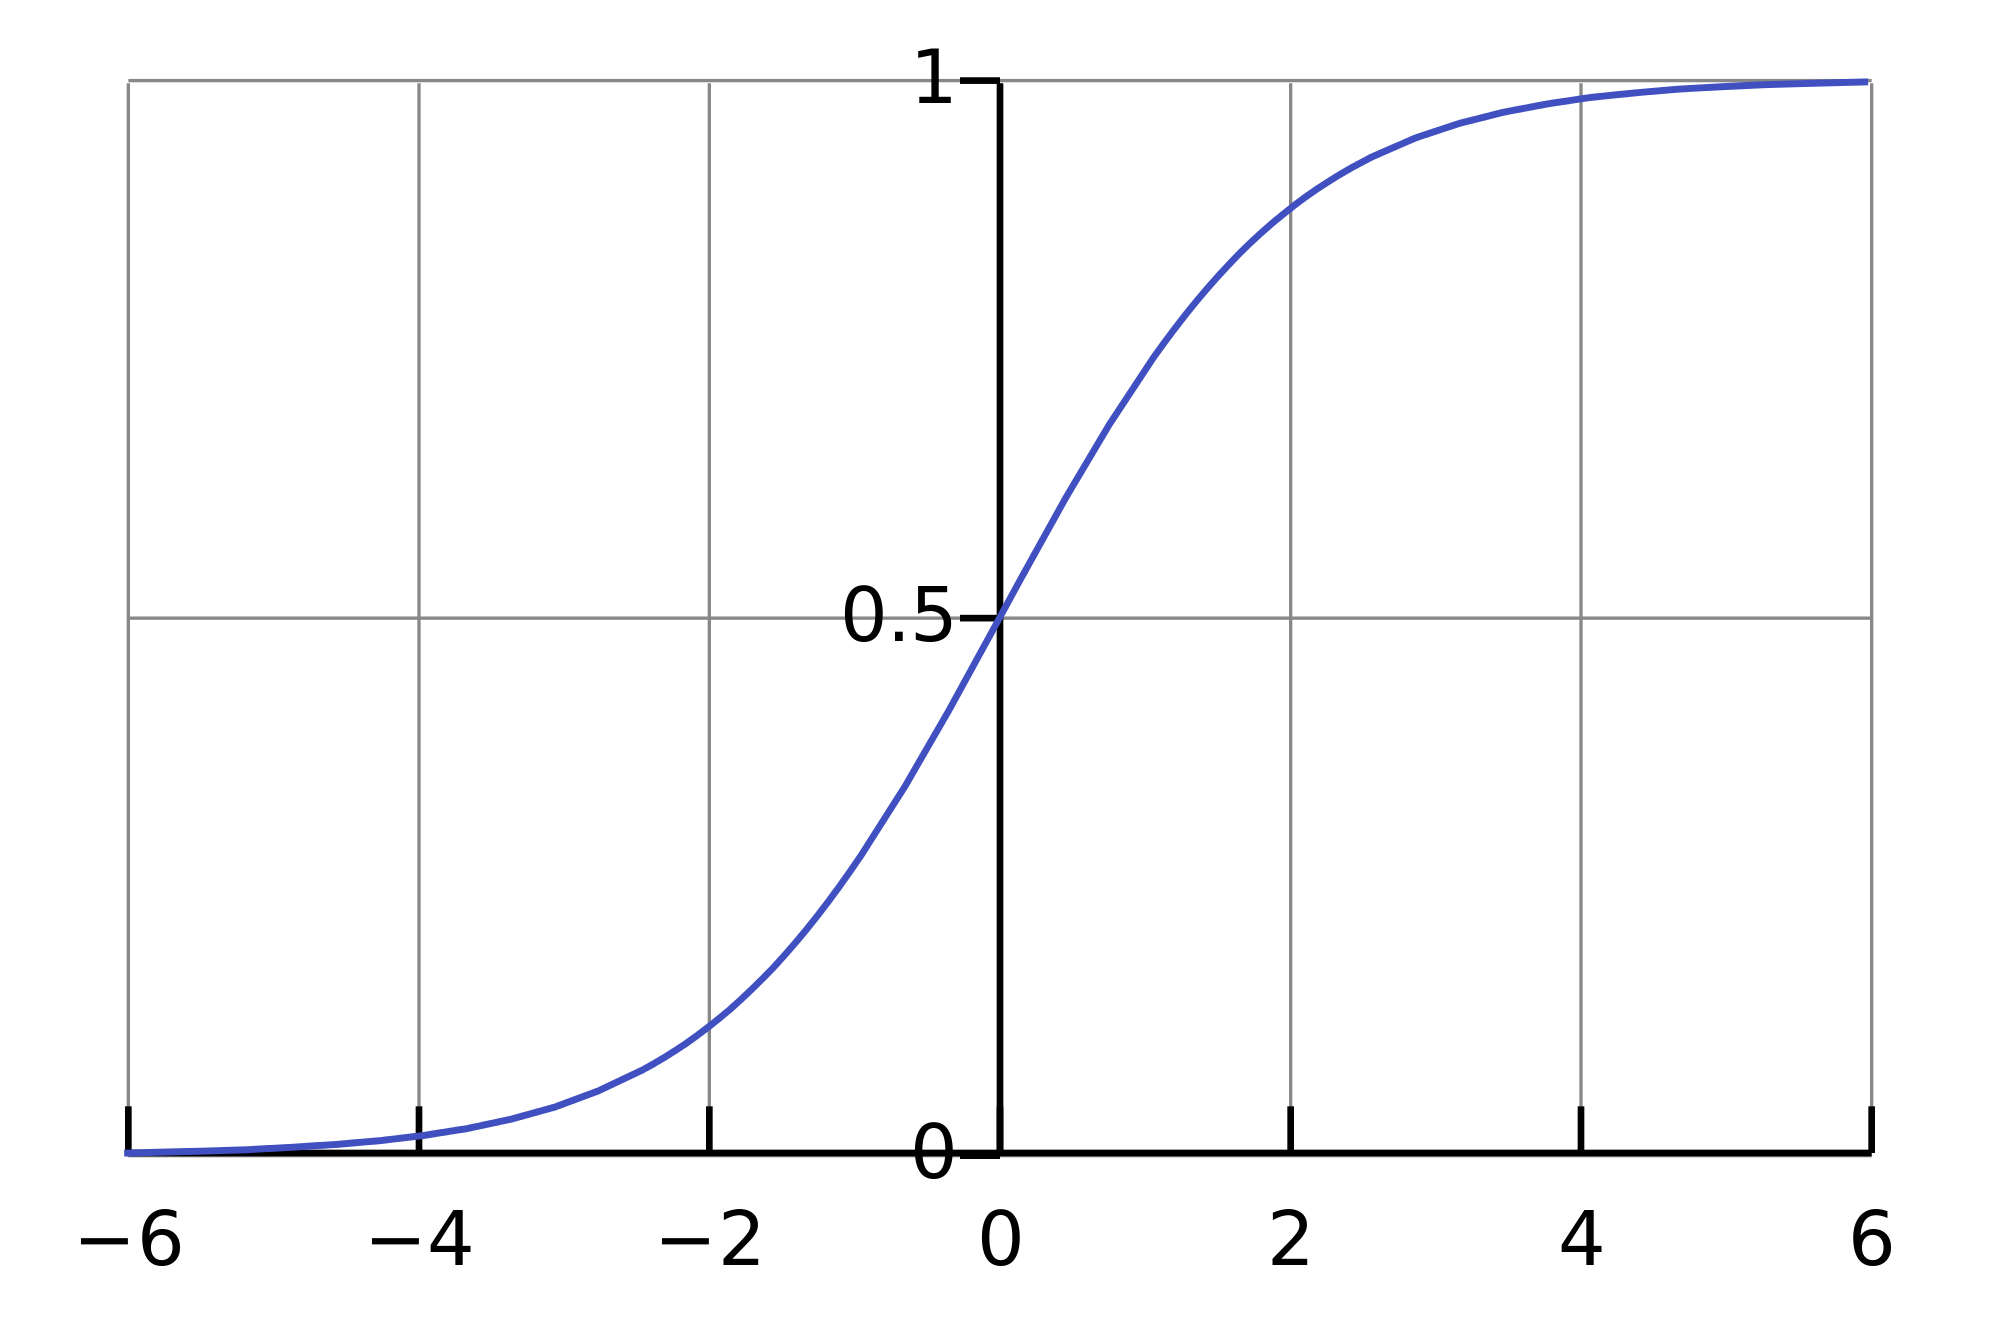
\includegraphics[width=0.95\linewidth]{../images/Logistic-curve.png}
	\caption{A graph of the logistic function.}
\end{figure}

\begin{equation}
% 	sigmoid(\inputVector,\weightMatrix,\basisVector)=\frac{1}{1+e^{-\weightMatrix\inputVector+\basisVector}}
	sigmoid(\inputVector)=\frac{1}{1+e^{-\inputVector}}
\end{equation}  

\begin{figure}
	\label{figure:tanh-function}
	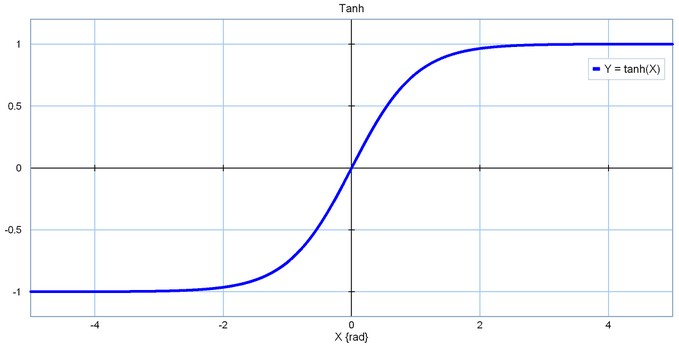
\includegraphics[width=0.95\linewidth]{../images/tanh_zoom60.jpg}
	\caption{A graph of the tanh function.}
\end{figure}

\begin{equation}
	tanh(\inputVector)=\frac
	{e^{\inputVector}-e^{-\inputVector}}
	{e^{\inputVector}+e^{-\inputVector}}
	%tanh(\inputVector,\weightMatrix,\basisVector)=\frac
	%{e^{\weightMatrix\inputVector+\basisVector}-e^{-\weightMatrix\inputVector+\basisVector}}
	%{e^{\weightMatrix\inputVector+\basisVector}+e^{-\weightMatrix\inputVector+\basisVector}}
\end{equation}


Often in RL the parameters of the model are denoted as \modelParameters and the goal is to optimize the bellman error with respect to these parameters. For logistic regression using the \textit{tanh} activation function this translates to $\modelParameters=\{\weightMatrix,\basisVector\}$. Where \weightMatrix are the weights for the model and \basisVector is a bias for the model. Somewhat similar to the more common $y=mx+b$ for defining a line. The \basisVector effectively shifts the curve to the right or left.

\section{Multidimensional Regression}

This model extends to multiple dimensions or \textit{actions} rather easily, $\inputVector, \basisVector$ become vectors and \weightMatrix is now a matrix with dimensions $len(\inputVector) x numActions$. Then the sigmoid function returns a vector of Q-values, one for each action in state \inputVector. The optimal action using the Q-Learning method can then be computed as

\begin{equation}
\action^{*}= \argmax_{\action}\qValueFunction{\state}{\action}{}= \argmax_{i} tanh(\state,\theta)
\end{equation}
Keep in mind that in the multidimensional case $tanh(x,\theta)$ returns a vector with a length equal to the number of actions for the actor. The index with the maximum value is chosen $\argmax tanh(x,\theta)$ and corresponds to the index for the best action to execute in state \state,

\subsection{Model Optimization}

To perform optimization using a tanh model a cost function is needed. The cost function is used to compute the difference between the current model and the perfect solution. For RL we use the Bellman Error to determine this
\begin{equation}
cost(R, S, S') = sum(0.5 * \delta(R, S, S')^{2})
\end{equation}
This cost function gives a fair measure of the model error. Note, in this formulation R,S,S′ are vectors or matrices and the squared the cost is used so that positive and negative errors to not cancel each other out in the sum. It is also common to use mean in this function instead of sum because sum is effected more by variable scale. Including our model in the cost function gives
\begin{equation}
cost(R, S, S', \theta) = sum(0.5 * \delta(R, S, S', \theta)^{2})
\end{equation}

To determine in what direction along the cost function contour will result in less error the gradient wrt the model parameters is needed 
$\frac{\partial cost}{\partial \modelParameters}$ in this case $\frac{\partial cost}{\partial \weightMatrix}, \frac{\partial cost}{\partial \basisVector}$ . This can be calculated in Theano rather easily.

\begin{lstlisting}
    g_W = T.grad(cost=cost, wrt=model.W)
    g_b = T.grad(cost=cost, wrt=model.b)
\end{lstlisting}

With the gradient in hand we can make a update rule to step in the direction of less cost.
\begin{equation}
	\weightMatrix' = \weightMatrix + (-\frac{\partial cost}{\partial \weightMatrix} \learningRate), 
	\basisVector' = \basisVector = (-\frac{\partial cost}{\partial \basisVector} \learningRate)
\end{equation} 

This can also be done in Theano rather simply as 

\begin{lstlisting}
updates = [(model.W, model.W + (-g_W * learning_rate),
           (model.b, model.b + (-g_b * learning_rate)]
\end{lstlisting}


Those are the steps needed to perform common Stochastic Gradient Descent (SGD). It should be noted that the \textit{learning rate} \learningRate for RL problems should be rather small, the effect of this will be discussed and shown later.
Model Training
Every time the agent selects an action a in some state s that leads to receiving some reward r and resulting in a new states s′ experience is gained. This single tuples of experience is kept in a experience history that is used to train the model. The experience history serves a similar purpose as training data in classification problems. 
Training the model (or updates) is done over a mini batch, where a mini batch is a randomly selected sample of from the experience history of the agent. 
Action Selection and Exploration
A common method to select an action to execute is e-greedy action selection. This algorithm simply selects one of the available actions at random with probability e. Otherwise, the selected action comes from the policy \(\pi(s)\), in this case the logistic regression model.

Learning Rate
One tough challenge that has only recently seen good solutions is deadling with highly eratic policy changes. The policy swings from one end of the spectrum to the other making it almost impossible for the optimization to eventually settle on a good policy.
Earlier I said we would look at the effect the learning rate has on the learning process. The learning rate is one of the parameters that influences the erraticness of the policy. The effect of a learning rate that is far to high is shown in the next two figures. Focus on the policy on the right that describes the optimal action/direction to be selected when the agent is in the location on the map that is the location of the arrow.


After lowering the learning rate from 0.5 to 0.01 small managable policy updates are made.

The Code 
Can be found here.

\begin{comment}
References:
1. https://en.wikipedia.org/wiki/Activation_function 
2. https://en.wikipedia.org/wiki/Q-learning 
3. http://deeplearning.net/software/theano/tutorial/examples.html#logistic-function 
4. http://deeplearning.net/tutorial/logreg.html#logreg 
5. https://webdocs.cs.ualberta.ca/~sutton/book/ebook/the-book.html 
\end{comment}


% \input{project_related_work}

% \input{project_gibbon_movement}

% \input{project_Conclusion}

% \section*{Acknowledgements}

\bibliographystyle{named}
\bibliography{project}

\end{document}
